%!TEX root = ../thesis.tex
%*******************************************************************************
%****************************** Third Chapter **********************************
%*******************************************************************************
\chapter{The influence of historical short-lived climate forcer emissions on aerosol properties and radiative forcing in UKESM1 CMIP6 simulations}
\label{ch3}
% **************************** Define Graphics Path **************************
\ifpdf
    \graphicspath{{Chapter3/Figs/Raster/}{Chapter3/Figs/PDF/}{Chapter3/Figs/}}
\else
    \graphicspath{{Chapter3/Figs/Vector/}{Chapter3/Figs/}}
\fi

% \emph{The results from this chapter were published in Atmospheric Chemistry and Physics in XXXX.}
% REF
% \emph{VS designed the study, analysed the results and wrote the manuscript. PTG
% and AA provided support for designing the study and analysing the results. All authors contributed
% to revising the manuscript.}


\section*{Abstract}
Motivation / general statement / grand challenge is TBD

Aerosol-cloud interactions are a source of uncertainty in climate predictions. Earth-systems models (ESM) increasingly feature online, i.e. fully-coupled, treatments of the interactions between chemistry, aerosols and clouds.  

Here we present an analysis of experiments performed with an ESM featuring a detailed two-moment, modal aerosol scheme and detailed atmospheric chemistry scheme that aim to quantify the role emissions changes and atmospheric oxidation on radiative forcing.

We use the histSST-piX performed using UKESM1.0 performed as part of the  Aerosol Chemistry Model Intercomparison (AerChemMIP) project from the Coupled-Model Intercomparison Project 6 (CMIP6) experiments. These experiments are designed to understand the role of changes in emissions of short-term climate forcers on the radiative balance of the atmosphere through transient, atmosphere-only experiments across the period 1850-2014, 

Here we present an analysis of the impact of changes in aerosol precursors, e.g.\ce{SO_2}, ozone precursors (e.g. \ce{NO_x} and \ce{CO}, and methane on aerosol formation, radiative forcing. We quantify the effect of changes in atmospheric oxidant levels, e.g. \ce{O_3} and \ce{OH}, on aerosol formation, and the impact on cloud properties and radiative forcing.

We find strong sensitivity to the levels of tropospheric OH, mediated by methane and ozone precursors, and impacts on aerosol nucleation rate, aerosol size distribution. The effect of historical increases methane, for example, lead to suppressed OH ?(XX\% lower) 
and lower nucleation rate, larger aerosols and lower cloud droplet number concentration (CDNC), with changes of around XX\% in OH. 
The effect of historical ozone precursor emissions changes is to enhance OH, with increased aerosol number concentration (XX\%). These emissions nearly completely offset each other in terms of OH, but the response of aerosols, clouds and forcing is more complex, with competing effects that on only partially counteract each other.

Other gas phase oxidants such as ozone and H2O2 also play significant roles (how much details). We show that these oxidants respond (to emissions of precursors, approx what drives O3 and H2O2) and have an impact (on stuff).   


1. How the emissions change in aerosol pre and O3 pre 
Role of methane important.

2. 40\% of the change in aerosol IRF from changes in oxidants at 2015

3. Sensitivity of the channels to the changes in emissions; SO2 oxidation by O3 not v sensitive to changes in O3 precursor, but oxidation by OH was.   


The impact bit

\section{Introduction}
Aerosols, micrometre-scale solid or liquid droplets suspended in the air, are an important group of climate forcing agents \citep{forsterEarthEnergyBudget2021}. Some aerosols can act to cool the climate via direct and indirect effects \citep{angstromAtmosphericTransmissionSun1929, twomeyInfluencePollutionShortwave1977, charlsonPerturbationNorthernHemisphere1991,szopaShortlivedClimateForcers2021}. However, the processes that control these effects are complex and represent our largest sources of uncertainty in modelling historic climate change \citep{ghanChallengesConstrainingAnthropogenic2016, forsterEarthEnergyBudget2021}.

% aerosol formation and SO2 emission
Aerosol can be emitted directly, e.g. black carbon, mineral dust and sea salt aerosols, and can be formed in situ through gas phase oxidation, e.g. sulfate and secondary organic aerosols, via the generation of aerosol precursors and subsequent nucleation \citep{prosperoAtmosphericAerosolSystem1983}. Sulfate aerosol is a significant type of climate-cooling aerosol which can be directly emitted into the atmosphere, but the vast majority of sulfate aerosol is formed in situ via oxidation of precursor sulfur gases, including sulfur dioxide (\ce{SO_2}), dimethyl sulfide and carbonyl sulfide \citep[e.g.][]{boucherGeneralCirculationModel1995, mulcahyDescriptionEvaluationAerosol2020}. Sources of \ce{SO_2} include anthropogenic emissions from fossil-fuel combustion, industrial activities and high-sulfur content fuel used in shipping \citep{hoeslyHistorical175020142018}, and biogenic sources such as volcanic activities and secondary production from dimethyl sulfide and carbonyl sulfide emitted by marine phytoplankton \citep{lanaUpdatedClimatologySurface2011}. Between 1990 and 2015, anthropogenic \ce{SO_2} emissions increased by 100 Tg(S) yr$^{-1}$ and became the most important source globally \citep{hoeslyHistorical175020142018, szopaShortlivedClimateForcers2021}.

% gas and aqueous oxidation  
The \ce{SO_2} reacts with multiple oxidants to form sulfate aerosols. The reaction between hydroxyl radical (\ce{OH}) and \ce{SO_2} leads to the gas phase production of sulfuric acid (\ce{H_2SO_4}), which can subsequently lead to new particle formation \citep{woodMechanismsAerosolFormation1975,mcmurryPhotochemicalAerosolFormation1980}. In cloud droplets, the dissolved SO2 (S(IV) = SO2·H2O + HSO3− + SO32−) is easily oxidized by H2O2, O3, hypohalous acids (HOX = HOCl + HOBr), and transition metal ions (TMI)-catalyzed O2 in the aqueous phase (Alexander et al., 2009; Chen et al., 2016), contributing to the growth of particles (Lelieveld \& Heintzenberg, 1992).


Sulfate aerosol formation is governed by a mix of the sources of \ce{SO_2} and oxidants. Modelling this is a challenge because the oxidants that \ce{SO_2} react with, \ce{OH}, \ce{H_2O_2} and \ce{O_3}, are controlled by complex chemical processes.  \ce{H_2O_2} is formed from \ce{HO_2} self-reaction, linking \ce{H_2O_2} concentration with \ce{OH} and \ce{HO_2} \citep{allenH2O2CH3OOHMHP2022}. OH is the atmosphere's primary oxidizing agent, but there is significant uncertainty in models' ability to reproduce recent trends in \ce{OH} compared with observationa bl estimates \citep{stevensonTrendsGlobalTropospheric2020}, as well as intermodel spread \citep{zhaoIntermodelComparisonGlobal2019,zhaoRoleTrendVariability2020,murrayLargeUncertaintiesGlobal2021}.

To understand the global aerosol-climate interaction, models with interactive sulfur cycles were developed \citep{langnerGlobalThreedimensionalModel1991, boucherCloudsAerosols2014}. This is then coupled with aerosol-cloud microphysics \citep[e.g. ][]{feichterSimulationTroposphericSulfur1996}. Finally, fully-coupled oxidant-aerosol-cloud treatment subsequently emerged \citep[e.g. ][]{tegenGlobalAerosolClimate2019, mulcahyUKESM1DevelopmentEvaluation2022}.

To address the complexity of this oxidant-aerosol-climate nexus, and represent the interactions more faithfully, climate models are increasingly coupling interactive gas-phase chemistry to aerosol formation \citep{tegenGlobalAerosolClimate2019, mulcahyDescriptionEvaluationAerosol2020}. The use of online oxidants in the description of aerosol is relatively new. Previous studies, using offline oxidants, have shown that oxidants are important in understanding the climate and in estimating aerosol radiative effects \citep{karsetStrongImpactsAerosol2018}.


The pathway that \ce{SO_2} is oxidised in the atmosphere will depend on where the \ce{SO_2} enters the atmosphere and the levels of the different oxidants it encounters \citep{roelofsAnalysisRegionalBudgets2001,yangImpactAnthropogenicEmission2019, wilcoxRegionalAerosolModel2022}. For example, emissions in the tropics will favour oxidation via OH, whereas the extratropics will favour reaction with \ce{O_3} and \ce{H_2O_2}, with these reactions known to be dependent on pH \citep{turnockImpactChangesCloud2019}. To improve the accuracy of climate models there is a need to model these processes faithfully. 


One of the areas that needs improvement is the aerosol radiative effect estimation. 
Aerosol radiative effects can be broken down into different components to tease out the radiative effect due to aerosol, clouds and others \citep{ghanChallengesConstrainingAnthropogenic2016}. Previous work has suggested that capturing the pre-industrial to present-day radiative forcing accurately requires models to simulate the change in the burden and size distribution of aerosols \citep{pilinisSensitivityDirectClimate1995, haywoodEstimatesDirectIndirect2000}. The latter is driven by the magnitude of emission changes, the former by a complex set of processes, including oxidation \citep{karsetStrongImpactsAerosol2018}. Furthermore, \citet{persadDivergentGlobalscaleTemperature2018} shows that geographic location substantially influences the cooling potential of a given aerosol emission. 

Moreover, greenhouse gases are shown to play an indirect role in aerosol formation and aerosol-cloud interactions by affecting oxidant levels. This effect is recently reported by \citet{oconnorApportionmentPreIndustrial2022} which shows that \ce{CH_4}, a greenhouse gas which is not an aerosol precursor, modifies aerosol particle formation and aerosol mass concentration.  % more here


AerChemMIP proposed a series of single forcing experiments where one component of the oxidant-aerosol-climate nexus was held constant at 1850 levels and all other drivers of the system were allowed to vary in a transient simulation from 1850-2014 \citep{collinsAerChemMIPQuantifyingEffects2017}. Here we examine the AerChemMIP transient historical prescribed sea-surface temperature experiments (histSSTs) runs which allow us to quantify the oxidants' effects on the evolution of aerosol ERF, a subject that has so far received little attention in the literature. The AerChemMIP experimental design complements the Climate Model Intercomparison Project Phase 6 (CMIP6) historical simulations by allowing the role of individual drivers of the changes in the coupled aerosol-oxidant-climate system to respond. By fixing \ce{CH_4} to pi levels (piCH4) the experiment allows for an increase in OH over time as increases in CH4 have lead to a depletion in OH \citep{zhaoRoleTrendVariability2020}. Similarly, fixing SO2 and other aerosol emissions (BC, OC etc) to 1850 levels (piAer) enables us to quantify the response of the system to the changes in aerosols only. The use of transient experiments enables us to examine the response of the system to the spatio-temporal evolution of anthropogenic emission sources, which have driven the changes since the pre-industrial era. 


In this paper, we use the AerChemMIP histSST simulations to investigate the effects of oxidant changes on sulfate aerosol formation, aerosol and cloud properties and aerosol effective radiative forcing. We investigate the time evolution of these processes due to changes in oxidants. In particular, we investigate the shift in aerosol size distribution over time due to oxidants which have a knock-on effect on aerosol effective radiative forcing. We examine the aerosol and cloud properties, and ultimately, aerosol ERF. 


The chapter is outlined as follows. The information about the model is presented in section 2.1. The oxidant chemistry in the model is described in section 2.1.1, followed by aerosol module description 2.1.2. The AerChemMIP simulation set-up is described in 2.2. Results and discussions are presented and discussed in section 3.

\section{Methods and data}

As described in Chapter \ref{ch2:title}, this work uses the UK's Earth System Model1, UKESM1 \citep{sellarUKESM1DescriptionEvaluation2019}, data provided for the AerChemMIP \citep{collinsAerChemMIPQuantifyingEffects2017} to examine the effects of \ce{SO_2} oxidation on radiative balance. 

Specifically this chapter examines the global properties of \ce{SO_2} oxidation, aerosol formation, cloud properties, and radiative effects. Concepts, simulations, and calculations that are unique to this chapter are described in detail below. The readier is kindly asked to refer to general details about the UKESM1 in Chapter \ref{ch2:title}.

\subsection{Experiment design: The Aerosol Chemistry Model Intercomparison Project}
\label{sec:aerchemmip}
The simulations used in this work were designed by the Aerosol Chemistry Model Intercomparison Project \citep[AerChemMIP;][]{collinsAerChemMIPQuantifyingEffects2017}. As part of the project, transient historical prescribed sea-surface temperature experiments (\textit{histSSTs}) were proposed to investigate transient ERFs. These simulations use atmosphere-only configurations with prescribed monthly mean sea-surface temperatures (SSTs) and sea ice taken from one ensemble member of the \textit{historical} simulation from the CMIP6 Diagnostic, Evaluation and Characterization of Klima (DECK) experiments \citep{eyringOverviewCoupledModel2016}. 


The experiment is set up as follows. The control simulation, \textit{histSST}, uses prescribed historical SSTs with all emissions set as is historical. The perturbed simulations have some of the emissions or concentrations set to the pre-industrial, i.e. 1850, level as shown in Table \ref{tab:histSST-exp} to determine its effect on the atmosphere. For example, \textit{histSST-piAer} has its aerosol precursor emissions set to pre-industrial levels. In this paper, we refer to \textit{histSST-piAer} as \textit{piAer}, \textit{histSST-piO3} as \textit{piO3}, and so on, for brevity. 


\begin{table}
   \caption[Emission for fixed-SST experiments]{A summary of emission configuration used in AerChemMIP transient fixed-SST experiments.}
   \label{tab:histSST-exp}
   \centering
   \begin{tabular}{l l l l l l}
     \hline\hline
     Experiment ID & \ce{CH_4}  & Aerosol precursors & \ce{O_3} precursors & Remarks \\
     \hline
     \textit{histSST}         & Hist & Hist & Hist & Historical experiment\\
     \textit{histSST-piAer}   & Hist & 1850 & Hist & Targets \ce{SO_2}\\
     \textit{histSST-piO3}    & Hist & Hist & 1850 & Targets \ce{O_3} \\
     \textit{histSST-piCH4}   & 1850 & Hist & Hist & Targets \ce{OH} \\
     \textit{histSST-piNTCF}  & Hist & 1850 & 1850 & Targets \ce{SO_2} and \ce{O_3}\\
     \hline\hline
   \end{tabular}
\end{table}


Some of the variables used in this study are archived on the WCRP database (https://esgf-index1.ceda.ac.uk/projects/esgf-ceda/), but we also employ native model data for the \ce{SO_2 - O_3} and \ce{SO_2 - H_2O_2} oxidation tendency, \ce{H_2O_2} mixing ratio, aerosol number mixing ratio by aerosol mode, aerosol mass mixing ratio by mode and component, and effective cloud droplet radius. Chemical lifetime, aerosol size distribution, aerosol concentration for particle size above 50 nm, and effective radiative forcing are derived values and are described below. See the Data Availability Section for more details.

\subsubsection{Emissions}
\label{sec:emissions}

\begin{figure}
    \centering
    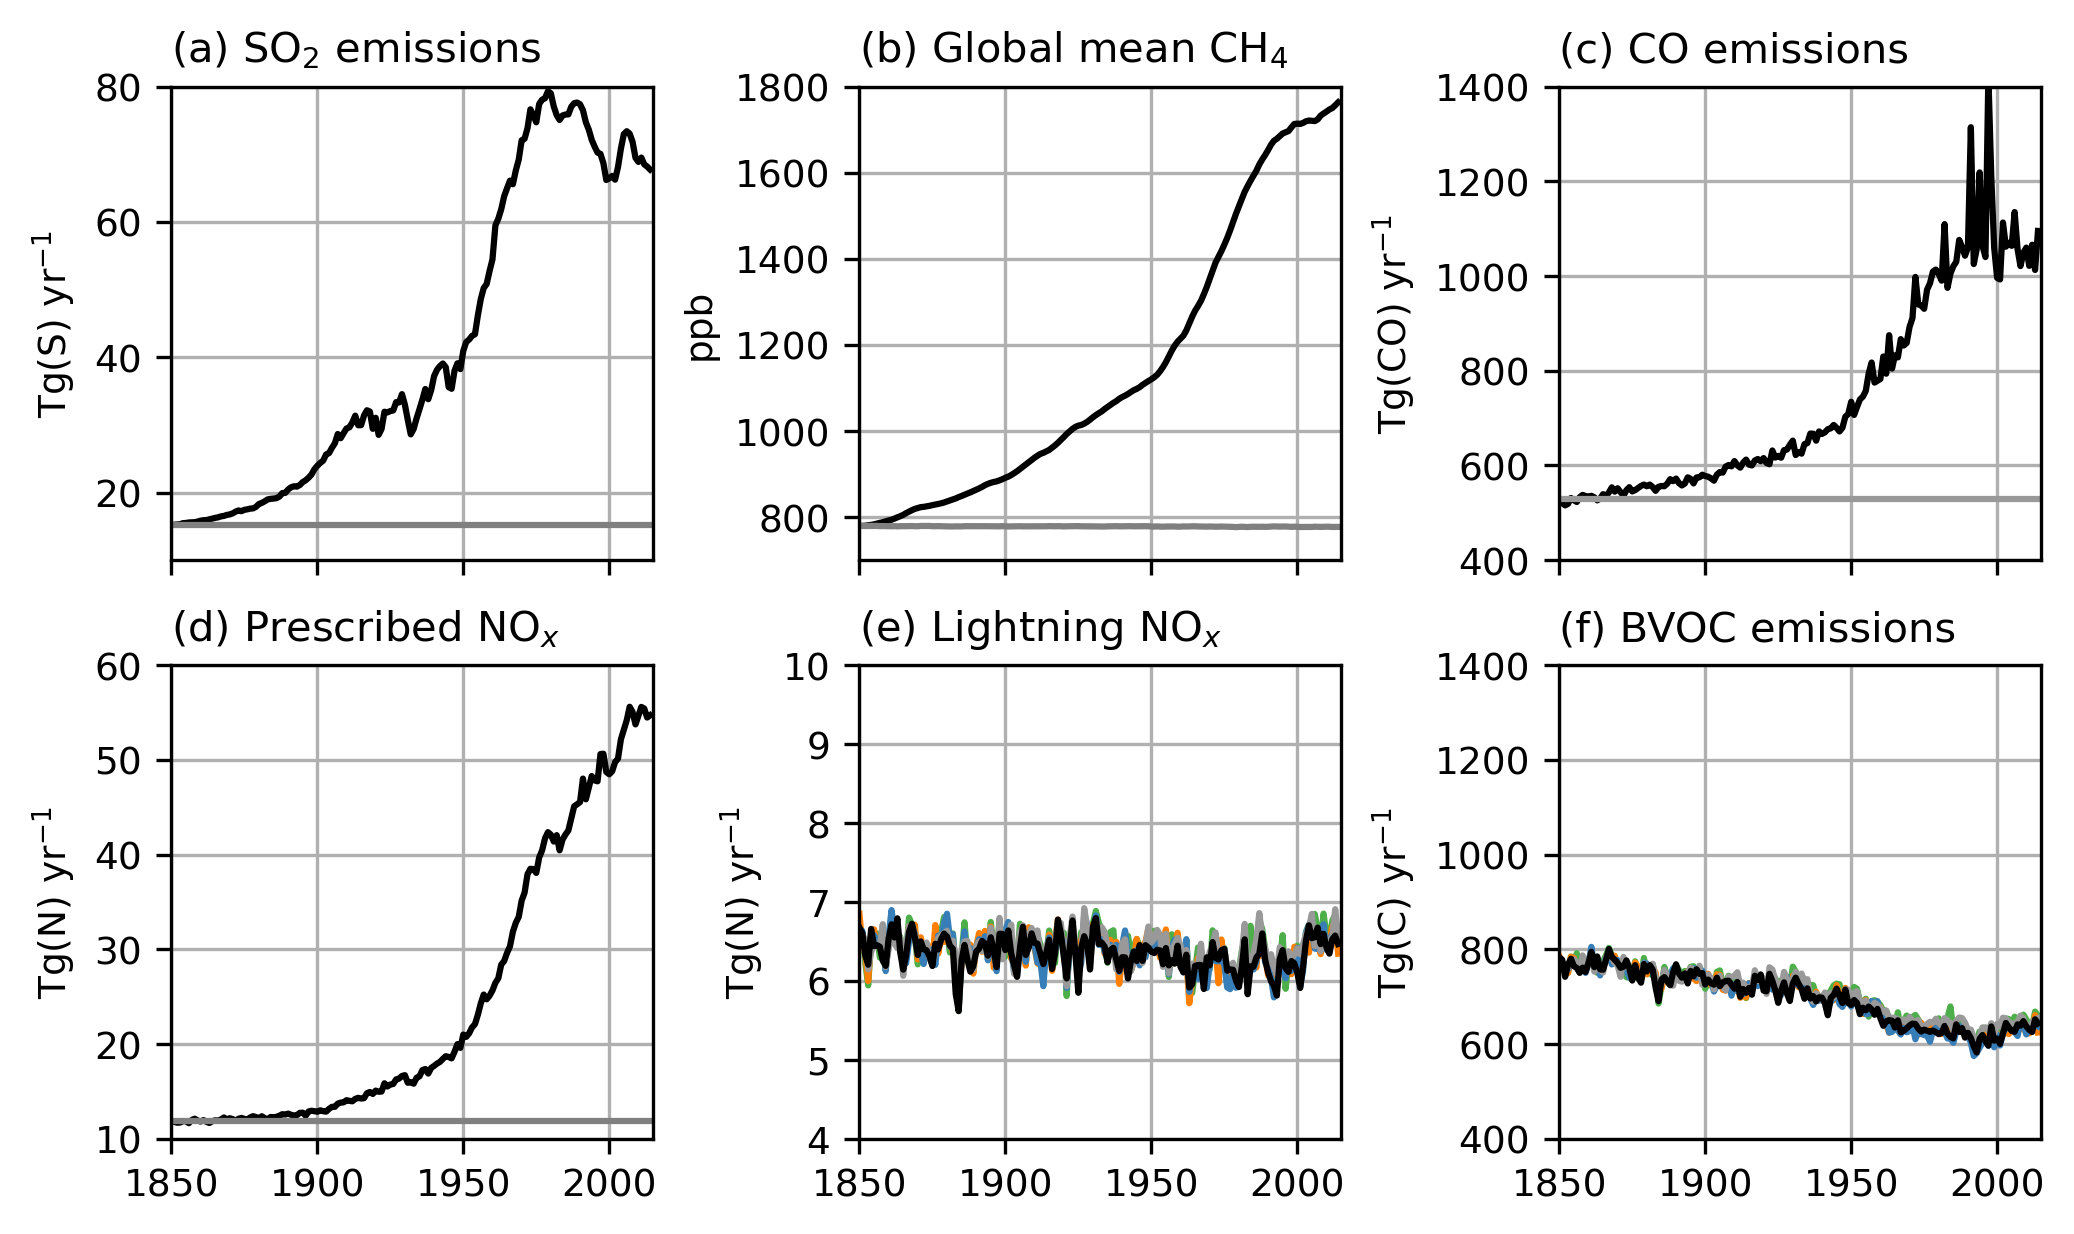
\includegraphics[width=\linewidth]{Chapter3/Figs/f01_emissions.png}
    \caption{Near-term climate forcer emissions and lower boundary conditions used to force simulations listed in Table \ref{tab:histSST-exp}. (a) Sulfur dioxide emissions include both natural and anthropogenic sources. (b) Methane concentration is constrained at the surface. Emissions of ozone precursors include (c) carbon monoxide, (d) prescribed \ce{NO_x} from surface and aircraft, (e) lightning \ce{NO_x}, and (f) biogenic volatile organic compounds (BVOCs). Lightning  \ce{NO_x} and BVOC are interactively simulated and are shown for each simulation.}
    \label{fig:emissions}
\end{figure}

Figure \ref{fig:emissions} shows the diagnosed emissions for \ce{SO_2}, \ce{O_3} precursor emissions including carbon monoxide (\ce{CO}), biogenic volatile organic compounds (BVOCs), nitric oxide (\ce{NO}) as \ce{NO_X}, and methane (\ce{CH_4}) concentration. 

\ce{O_3} precursors including surface \ce{NO_x}, lightning \ce{NO_x}, \ce{CO} and biogenic volatile organic compounds (BVOCs) emissions are calculated from the \textit{eminox}, \textit{emilnox}, \textit{emico}, and \textit{emibvoc} variables, respectively. The \textit{eminox} variable is the sum of anthropogenic, biomass burning, soil and aircraft \ce{NO_x}. Biomass burning contributes 6.4 Tg(N) yr$^{-1}$ and soil contributes 5.6 Tg(N) yr$^{-1}$ \citep{archibaldDescriptionEvaluationUKCA2020}. Anthropogenic \ce{NO_X} increases from 0 to 40.2 Tg(N) yr$^{-1}$ between 1850 and 2015. 

\ce{CH_4} concentration is taken from variable \textit{ch4}. The UKESM1 constrains lower boundary conditions for \ce{CH_4}. Since \ce{CH_4} has a lifetime of 8.1-9.8 years \citep{oconnorAssessmentPreindustrialPresentday2021}, it is well-mixed across the atmosphere. Figure 1 shows that global \ce{CH_4} concentration has increased monotonically over time since the 1850s.

Total \ce{SO_2} emissions are calculated from the \textit{emiso2} variable. This includes both volcanic and anthropogenic \ce{SO_2} emissions but does not include secondary production from dimethyl sulfide. 

Figure 1 shows that historical changes in NOx emissions are driven by changes in ANOx at the surface.  Isoprene declines - effect on OH and O3, non-linearity in Stevenson 2020.

\section{Results and discussions}
\label{sec:results}

\subsection{Oxidant changes due to near-term climate forcing}
\begin{figure}
    \centering
    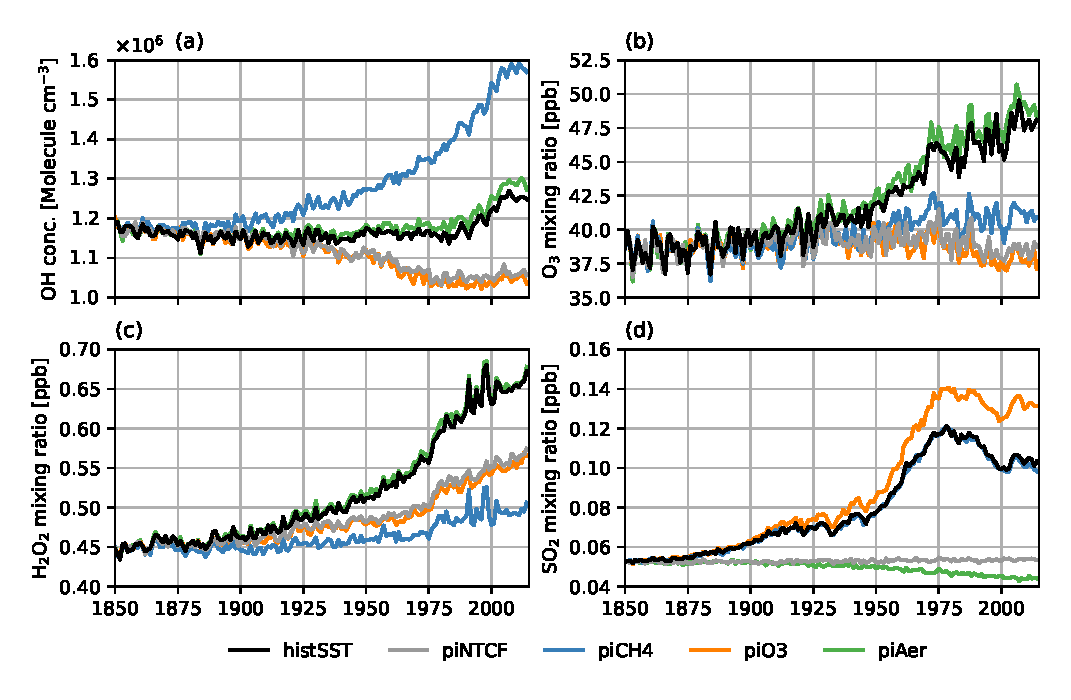
\includegraphics[width=\linewidth]{Chapter3/Figs/f02_oxidant-changes.eps}
    \caption{Global annual mean tropospheric oxidant concentration or mixing ratio for species related to \ce{SO_2} oxidation in each experiment as mentioned in Table \ref{tab:histSST-exp}}
    \label{fig:f02}
\end{figure}

Available oxidants play an important role in controlling the oxidation rate. Figure \ref{fig:f02} shows global annual mean of tropospheric oxidants that influence \ce{SO_2} oxidation, including \ce{OH}, \ce{O_3}, \ce{H_2O_2} and \ce{SO_2}. It shows that the \ce{SO_2} mixing ratio follows the \ce{SO_2} emission trends (Figure \ref{fig:emissions}) with the maximum mixing ratio increasing by two times that of the 1850s.  \ce{O_3} precursor emissions increase the \ce{SO_2} mixing ratio by 27.5\% (from 0.10 to 0.13 ppb) as the decrease in oxidants in the counterfactual decreases the chemical sink of \ce{SO_2}. 


\ce{O_3} mixing ratio is controlled by \ce{O_3} precursor emissions and also \ce{CH_4}. Comparing histSST with piO3 in Figure \ref{fig:f02}c, the \ce{O_3} mixing ratios show an increase in the historical period with the main source of \ce{O_3} coming from \ce{O_3} precursors including \ce{NO_x}, \ce{CO} and biogenic volatile organic compounds, all of which shows a monotonic increase since 1850 \citep{griffithsTroposphericOzoneCMIP62021}. \ce{CH_4} is another source of \ce{O_3} as \ce{CH_4} forms \ce{CH_3O_2} which reacts with \ce{NO} to form formaldehyde (\ce{HCHO}). \ce{HCHO} photolysis yields \ce{CO} which is a source of tropospheric \ce{O_3}. Keeping \ce{CH_4} at 1850 level decreases tropospheric \ce{O_3} as shown in the Figure \ref{fig:f02}c.


\ce{OH} concentrations remain constant until 1975 and increase by 0.1$\times 10^6$ cm$^{-3}$ by the end of 2014 in the historical trajectory (histSST). The lack of increase in \ce{O_3} precursor emissions lowers OH concentration by 15\% (from 1.25$\times10^6$ to 1.05$\times10^6$ molecules cm$^{-3}$) as shown in piO3 and piNTCF compared to the historical trajectory. This decrease is due to less OH production by the reaction of water vapour with excited oxygen atoms \ce{(O(^1D))}, which are produced by \ce{O_3} photolysis ($\lambda$ < 340 nm). In contrast, for piCH4, where \ce{CH_4} concentration is held at the 1850 level, \ce{OH} concentrations increase above the historical trajectory. We expect that, in this case,  OH production rates are lower, due to lower \ce{O_3} in this experiment, but that in the absence of an increase in \ce{CH_4} levels, the OH sink via OH+CH4 is smaller in piCH4 than in histSST. Overall, the effect of historical increases in CH4, is seen as an increase in OH. The effect of historical increases in  \ce{CH_4} on OH can be seen since 1875 with the \ce{OH} concentration in 2014 increasing to 133\% that of 1850. 


\ce{H_2O_2} burden increases after 1850, with a larger increment in \textit{histSST}, which could be attributed to NTCF emissions and sea surface temperature (SST). Keeping \ce{CH_4} at 1850 levels decreases \ce{H_2O_2} levels as \ce{CH_4} is a source of \ce{HO_2} radicals, via reactions that form \ce{HCHO} and \ce{HO_2} radicals (and hence \ce{H_2O_2}). \ce{H_2O_2} is also contributed by \ce{CO}, an \ce{O_3} precursor, via its reaction with \ce{OH} to form \ce{HO_2}. 


The historical changes of all oxidants are subject to the uncertainty of their sources and chemical processes included in the model. It has been reported that \ce{SO_2} emissions over China in CMIP6 deviate from the bottom-up, country-level inventory after 2005 \citep{fanComparisonAnthropogenicEmission2022}. This will affect the accuracy of the \ce{SO_2} mixing ratio and consequently the oxidation downstream. The recent rise in \ce{OH} concentration is also observed in other climate models \citep{zhaoIntermodelComparisonGlobal2019}. 


While anthropogenic \ce{SO_2} emissions play a large role in the overall budget, natural emissions are not negligible. However, the AerChemMIP simulation we employed does not archive the secondary natural \ce{SO_2} emissions from dimethyl sulfide oxidation, but this is reported in The UKESM1 18-year AMIP simulation \citep{mulcahyDescriptionEvaluationAerosol2020}. The Atmospheric Model Intercomparison Project (AMIP) is an atmosphere-only configuration for detailed aerosol budget analysis driven by observed sea surface temperature (SST) and sea ice. This has additional diagnostics were not output in the historical simulations or the transient AerChemMIP we utilised. It reported the emission rate for anthropogenic, primary and secondary natural \ce{SO_2} emissions as 60.6, 14.06 and 16.69 Tg(S) yr$^{-1}$, respectively \citep{mulcahyDescriptionEvaluationAerosol2020}. 

%discuss change to oxidation if ph is changed in Tunnock

To summarise this section, historical \ce{O_3} precursor emissions promote \ce{OH} concentration, \ce{O_3} and \ce{H_2O_2} mixing ratio. The historical \ce{CH_4} reacts away \ce{OH} but boosts \ce{O_3} and \ce{H_2O_2}. The \ce{SO_2} emissions from aerosol precursors increase \ce{SO_2} mixing ratio as its main anthropogenic source.

\subsection{\ce{SO_2} oxidation and budget changes due to NTCF precursor emissions}

\subsubsection{\ce{SO_2} oxidation}
\label{sec:oxidation}


\begin{figure}
    \centering
    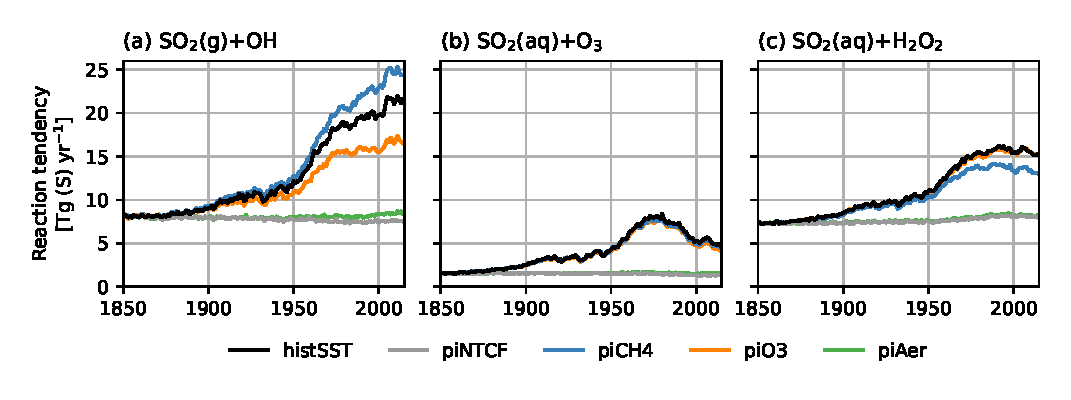
\includegraphics[width=\linewidth]{Chapter3/Figs/f03_oxidation.eps}
    \caption{Global annual \ce{SO_2} oxidation tendencies between 1850-2014 with changes due to constraining  methane concentration (piCH4), aerosol precursors (piAer), ozone precursors (piO3) or both emissions (piNTCF) at 1850 level.}
    \label{fig:f03}
\end{figure}


In the UKESM1, \ce{SO_2} reacts with \ce{OH} in the gas phase and with \ce{H_2O_2} and \ce{O_3} in the aqueous phase to form sulfate aerosols. Figure \ref{fig:f03} shows total annual tropospheric \ce{SO_2} oxidation tendencies in each pathway. In the historical period, \ce{SO_2} oxidation by \ce{OH} is the largest of the three pathways, contributing 20 Tg(S) yr$^{-1}$ globally in 2014. The \ce{SO_2+OH} trend broadly follows the \ce{SO_2} emissions and the \ce{OH} concentration trends. The lower \ce{OH} concentration decreases \ce{SO_2+OH} reaction tendencies in piO3, and, similarly, the increase in OH concentration in piCH4 enhances \ce{SO_2-OH} reaction tendencies.

\ce{SO_2 + O_3} reaction tendencies, however, are not sensitive to changes in \ce{O_3} mixing ratios. Figure \ref{fig:f02}b shows that the global \ce{O_3} mixing ratio monotonically increases after 1850, but historical \ce{SO_2 + O_3} does not share the trend. As a result of anthropogenic \ce{O_3} precursor emissions being fixed at the 1850 level in piO3, the \ce{O_3} concentration is lower than that of histSST. Despite the 25\% decrease in \ce{O_3} mixing ratio in piO3 and piCH4, there are minimal changes to \ce{SO_2 - O_3} tendencies in these experiments compared to \textit{histSST}. The lack of change implies that globally \ce{SO_2 - O_3} oxidation is not sensitive to historical changes in \ce{O_3} and that the background tropospheric \ce{O_3} is sufficient to saturate the pathway. 

\ce{SO_2 + H_2O_2} oxidation tendencies follow the \ce{SO_2} emissions and \ce{H_2O_2} mixing ratio trends. The historical oxidation tendency starts at 7.5 Tg(S) yr$^{-1}$ and increases to 16 Tg(S) yr$^{-1}$ and stabilises after the 1980s. The \ce{SO_2 - H_2O_2} reaction tendencies decrease by 15\% when the \ce{H_2O_2} mixing ratio decreases in the absence of anthropogenic \ce{CH_4} which is a source of \ce{H_2O_2} precursor. 


While past measurements and laboratory research have determined that only \ce{OH} is important for the oxidation of \ce{SO_2} in the gas phase during daytime \citep[][and reference therein]{rattiganUptakeGasphaseSO22000, eatoughConversionSO2Sulfate1994}, heterogeneous and aqueous-phase oxidation is more complex with multiple competing oxidants and aerosol properties at play \citep{pattantyusReviewSulfurDioxide2018, seinfeldAtmosphericChemistryPhysics2016}. \citet{seinfeldAtmosphericChemistryPhysics2016} mentioned the oxidation of S(IV) by organic peroxides, and iron and manganese as catalysts to oxygen. A further mechanism for \ce{SO_2} oxidation in solution with sea water is proposed via halogen compounds \ce{HOCl} and \ce{HOBr} in the remote marine boundary layer \citep{vogtMechanismHalogenRelease1996}. Aside from oxidation with \ce{OH}, \ce{O_3} and \ce{H_2O_2}, these further mechanisms are not included in the UKESM1 so are not considered in this study. 


Overall, the rate of \ce{SO_2} oxidation with \ce{OH}, \ce{O_3} and \ce{H_2O_2} is controlled by \ce{SO_2} abundance, as the reaction tendency tends to be constant over time without aerosol precursor emissions (green line in Figure \ref{fig:f03}). The \ce{OH} and \ce{H_2O_2} pathways contribute equally to \ce{SO_2} oxidation in the 1850s but the rate of growth of \ce{SO_2 + OH} oxidation is greater post-1950s, making \ce{SO_2 + OH} the most important oxidising pathway. \ce{O_3} is the least important oxidant globally, contributing to the removal of at most 8 Tg(S) yr$^{-1}$. Overall, Figure \ref{fig:f03} shows that the \ce{SO_2 + OH} pathway is the most sensitive to oxidant changes in which the spread between piO3 and piCH4 is ~ 5Tg S yr$^{-1}$ or 25\% of the histSST oxidation rate at 2014.



\subsubsection{\ce{SO_2} and \ce{SO_4} burden, losses and budgets}

\begin{figure}
    \centering
    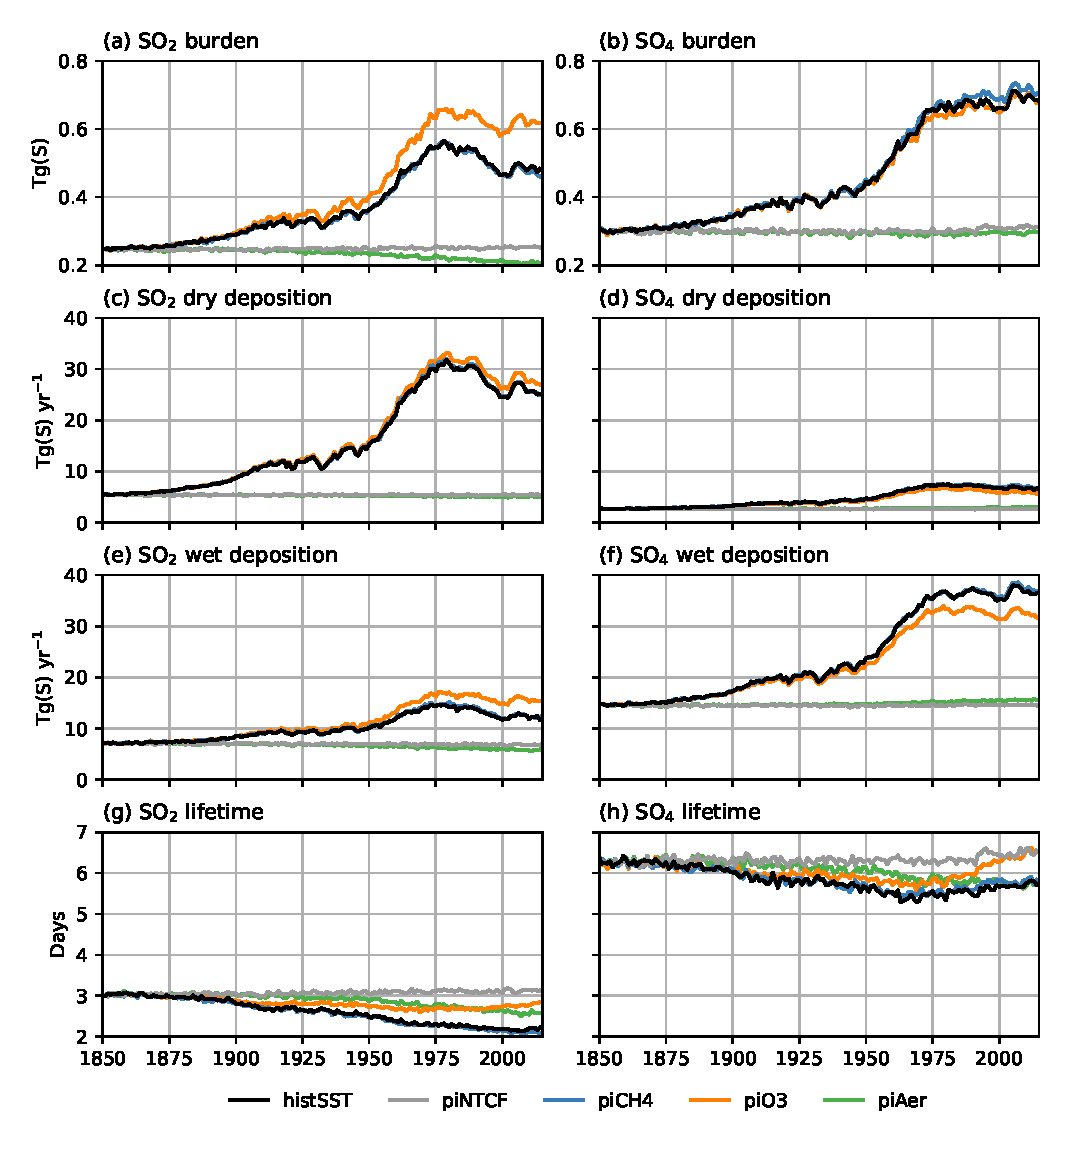
\includegraphics[width=\linewidth]{Chapter3/Figs/f04_s-budget.eps}
    \caption{Tropospheric \ce{SO_2} and \ce{SO_4} budget, including (a-b) burdens, (c-d) dry depositions, (e-f) wet depositions, and (g-h) lifetimes. The plots show budget terms between 1850-2014 with changes due to constraining  methane concentration (piCH4), aerosol precursors (piAer), ozone precursors (piO3) or both emissions (piNTCF) at the 1850 level.}
    \label{fig:f04}
\end{figure}

\ce{SO_2} reacts with \ce{OH}, \ce{H_2O_2} and \ce{O_3} to form sulfate (\ce{SO_4}) so the budget of \ce{SO_2} and \ce{SO_4} are linked via these oxidation processes. Figure \ref{fig:f04} shows that the \ce{SO_2} burden trend follows that of \ce{SO_2} emissions. \ce{SO_2} is lost mainly by oxidation (45 Tg(S) yr$^{-1}$ in 2014) followed by dry deposition (28 Tg(S) yr$^{-1}$). The lifetime of \ce{SO_2} is 3 days in the 1850s and decreases to 2.8 days in 2014. 

Oxidants affect the \ce{SO_2} budget in various ways. The lifetime of a trace gas describes how long it stays in the atmosphere and is defined as the average time that a molecule of that species remains in a reservoir before removal. If the reservoir is the whole atmosphere and is in a steady state, that is the burden is considered constant, and the tropospheric lifetime of a compound is estimated by dividing the total tropospheric burden by total loss. \ce{SO_2} loss terms include chemical losses via oxidation with \ce{OH}, \ce{O_3}, and \ce{H_2O_2}, wet and dry deposition. \ce{SO_4} is lost only via wet and dry deposition.

The lower levels of \ce{O_3} in piO3 result in less \ce{OH}, which leads to a smaller \ce{SO_2} sink than in histSST. This increases the \ce{SO_2} burden, dry and wet deposition and ultimately leads to a longer lifetime. This change to the \ce{SO_2} budget due to lower \ce{O_3} is also seen in piAer and piNTCF where \ce{SO_2} is kept at the 1850 level throughout the historical period. In piNTCF, in which \ce{O_3} precursor emissions are kept at the 1850 level (low \ce{O_3}), the \ce{SO_2} burden, wet and dry deposition and lifetime are lower compared to the case that \ce{O_3} precursors follow the historical trajectory (piAer). This further indicates the role of \ce{O_3} in the \ce{SO_2} budget via oxidation with \ce{OH}.


In contrast to piO3, where the lower \ce{O_3} and oxidant levels increase \ce{SO_2}, the piCH4 run shows that the SO2 burden stays roughly the same as the histSST run, despite the huge differences in \ce{CH_4} and as a result OH (see Figure \ref{fig:emissions}). This is because whilst there is a significant increase in \ce{SO_2 + OH} oxidation in piCH4, this is nullified by the decrease in \ce{SO_2 + H_2O_2} oxidation as seen in figure \ref{fig:f03}a and c. In this case, the \ce{SO_2} lifetime remains unchanged compared with the histSST.

Figure \ref{fig:f04} shows that, in piO3, exposing \ce{SO_2} emissions to pre-industrial \ce{O_3} increases the lifetime of both \ce{SO_2} and \ce{SO_4}. The effect of oxidant changes to \ce{SO_2} lifetime was observed in a modelled study by \citep{karsetStrongImpactsAerosol2018}. They found that by replacing oxidants (\ce{NO_3}, \ce{O_3}, \ce{OH} and \ce{HO_2}) from present-day to pre-industrial, the lifetime of pre-industrial \ce{SO_2} increases from 29 hours (1.21 days) to 34 hours (1.42 days), which is an increase by 17\%. In this work, the \ce{SO_2} lifetime increases by 28\% (from 2.17 days to 2.77 days). As aerosol has a longer lifetime, they are transported higher up in the atmosphere before getting oxidised, making it less likely to be removed by deposition. The dry deposition of the newly formed nucleation mode \ce{SO_4} decreased by 2.6\%. 

The \ce{SO_4} burden is generally higher than that of \ce{SO_2} because of its longer lifetime. The \ce{SO_4} burden has increased from 0.3 to 0.7 Tg(S) yr$^{-1}$ between 1850 and 2014. Because UKESM1 treats \ce{SO_4} as an aqueous aerosol, the primary removal process for \ce{SO_4} is wet deposition. The lifetime of \ce{SO_4} is 5.5-6 days which is double that of \ce{SO_2}. Changes in oxidants have a knock-on effect on \ce{SO_4} budget and lifetime. In piO3 where anthropogenic \ce{O_3} is missing, there is less \ce{SO_4} wet deposition as there is less conversion from \ce{SO_2} to \ce{SO_4} and more physical removal of \ce{SO_2} (via both wet and dry deposition). This reduction in \ce{O_3} and oxidants in piO3 also results in an increase in \ce{SO_4} lifetime compared to histSST. 


The budget report in our work is comparable to that reported by the UKESM1 evaluation using AMIP simulation covering 1981-1998 \citep{mulcahyDescriptionEvaluationAerosol2020}. The AMIP \ce{SO_2} and \ce{SO_4} are 0.53 and 0.67 Tg(S), respectively, the same as our values. For dry deposition, the AMIP values for \ce{SO_2} and \ce{SO_4} are 28.98 and 7.10 Tg(S) yr$^{-1}$, comparable to that of ours of 28.90 and 7.13 Tg(S) yr$^{-1}$. As for the wet deposition, the AMIP reported 13.38 and 36.0 Tg(S) yr$^{-1}$ for \ce{SO_2} and \ce{SO_4}, while our results are 13.47 and 36.40 Tg(S) yr$^{-1}$. Finally, the AMIP lifetime of \ce{SO_2} and \ce{SO_4} are 2.08 and 5.56 days, respectively, which are comparable to our work (2.23 and 5.56 days).  

The UKESM1 has been evaluated against both ground-based measurements and field campaigns \citep[e.g.][]{griffithsTroposphericOzoneCMIP62021, russoSeasonalInterannualDecadal2023}. The UKESM1 CMIP6 simulations capture the \ce{SO_4} trends compared to ground-based measurements, according to \citet{mulcahyDescriptionEvaluationAerosol2020}. The observed decreasing trend in \ce{SO_4} concentration across Europe is reproduced by the model. Although there is a consistent underprediction of the absolute values for all years, the model prediction sits within the observed variability. The UKESM1 overestimated \ce{SO_2} concentration compared to the Atmospheric Tomography (ATom) field campaign which measures atmospheric constituents and chemical processes in marine remote areas across both hemispheres \citep{ranjithkumarConstraintsGlobalAerosol2021}. \citet{ranjithkumarConstraintsGlobalAerosol2021} found that the UKESM1 model overestimated \ce{SO_2} concentration by approximately a factor 2–6 in the boundary layer regions of the tropics and mid-latitudes and the tropical upper troposphere. The biases in the upper-tropospheric mid and high latitudes are negligible. This may imply that the \ce{SO_2} removal process is underestimated or that the natural secondary emissions from DMS are overestimated.  

An in-depth evaluation has shown that the UKESM1 underestimated the dry deposition process and there has been an update released for the model to amend for this error \citep{hardacreEvaluationSO2SO422021}. Model evaluation against ground-based measurements shows that while the UKESM1 captures historical trends for decreasing the concentration of \ce{SO_2} and \ce{SO_4}, it overpredicts \ce{SO_2 by} a factor of 3 and underpredicted surface \ce{SO_4} by 25-35\% \citep{hardacreEvaluationSO2SO422021}. This has led to an update to the UKESM1 configuration called the UKESM1.1 \citep{mulcahyUKESM1DevelopmentEvaluation2022}. When a more realistic dry deposition scheme is implemented, it reduces the model’s overprediction of surface \ce{SO_2} concentrations and total column \ce{SO_2} but also decreases the overall \ce{SO_4} loading, exacerbating the low bias.  Our study used the original UKESM1 thus the overestimation of \ce{SO_2} is expected.



\subsection{Aerosol properties}

\subsection{Aerosol optical depth}

\begin{figure}
    \centering
    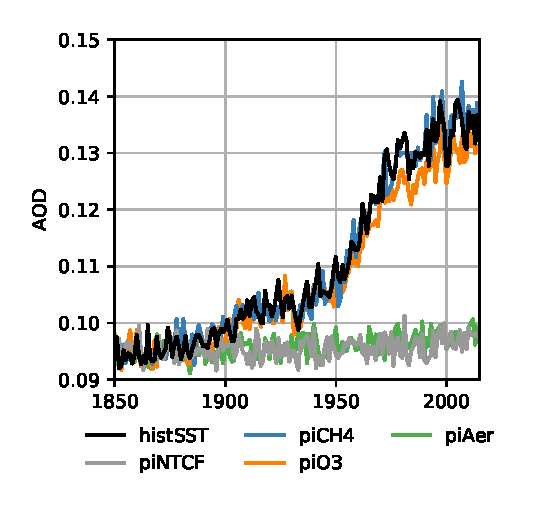
\includegraphics[width=0.5\linewidth]{Chapter3/Figs/f05_aod-trend.eps}
    \caption{Global annual mean aerosol AOD between 1850-2014 with changes due to constraining  methane concentration (piCH4), aerosol precursors (piAer), ozone precursors (piO3) or both emissions (piNTCF) at 1850 level.}
    \label{fig:AOD}
\end{figure}


The amount of aerosol in the atmosphere is linked to \ce{SO_2} oxidation tendency as it produces \ce{SO_4} aerosols. Figure \ref{fig:AOD} shows annual global mean AOD from different experiments. It shows that aerosol precursors increase AOD by 50\% and are the main contributor to global AOD. AOD in the piO3 experiment is lower than histSST by 0.05, suggesting that ozone contributes to some aerosol formation. Global AOD is unchanged under lower \ce{CH_4} condition in piCH4.

\begin{figure}
    \centering
    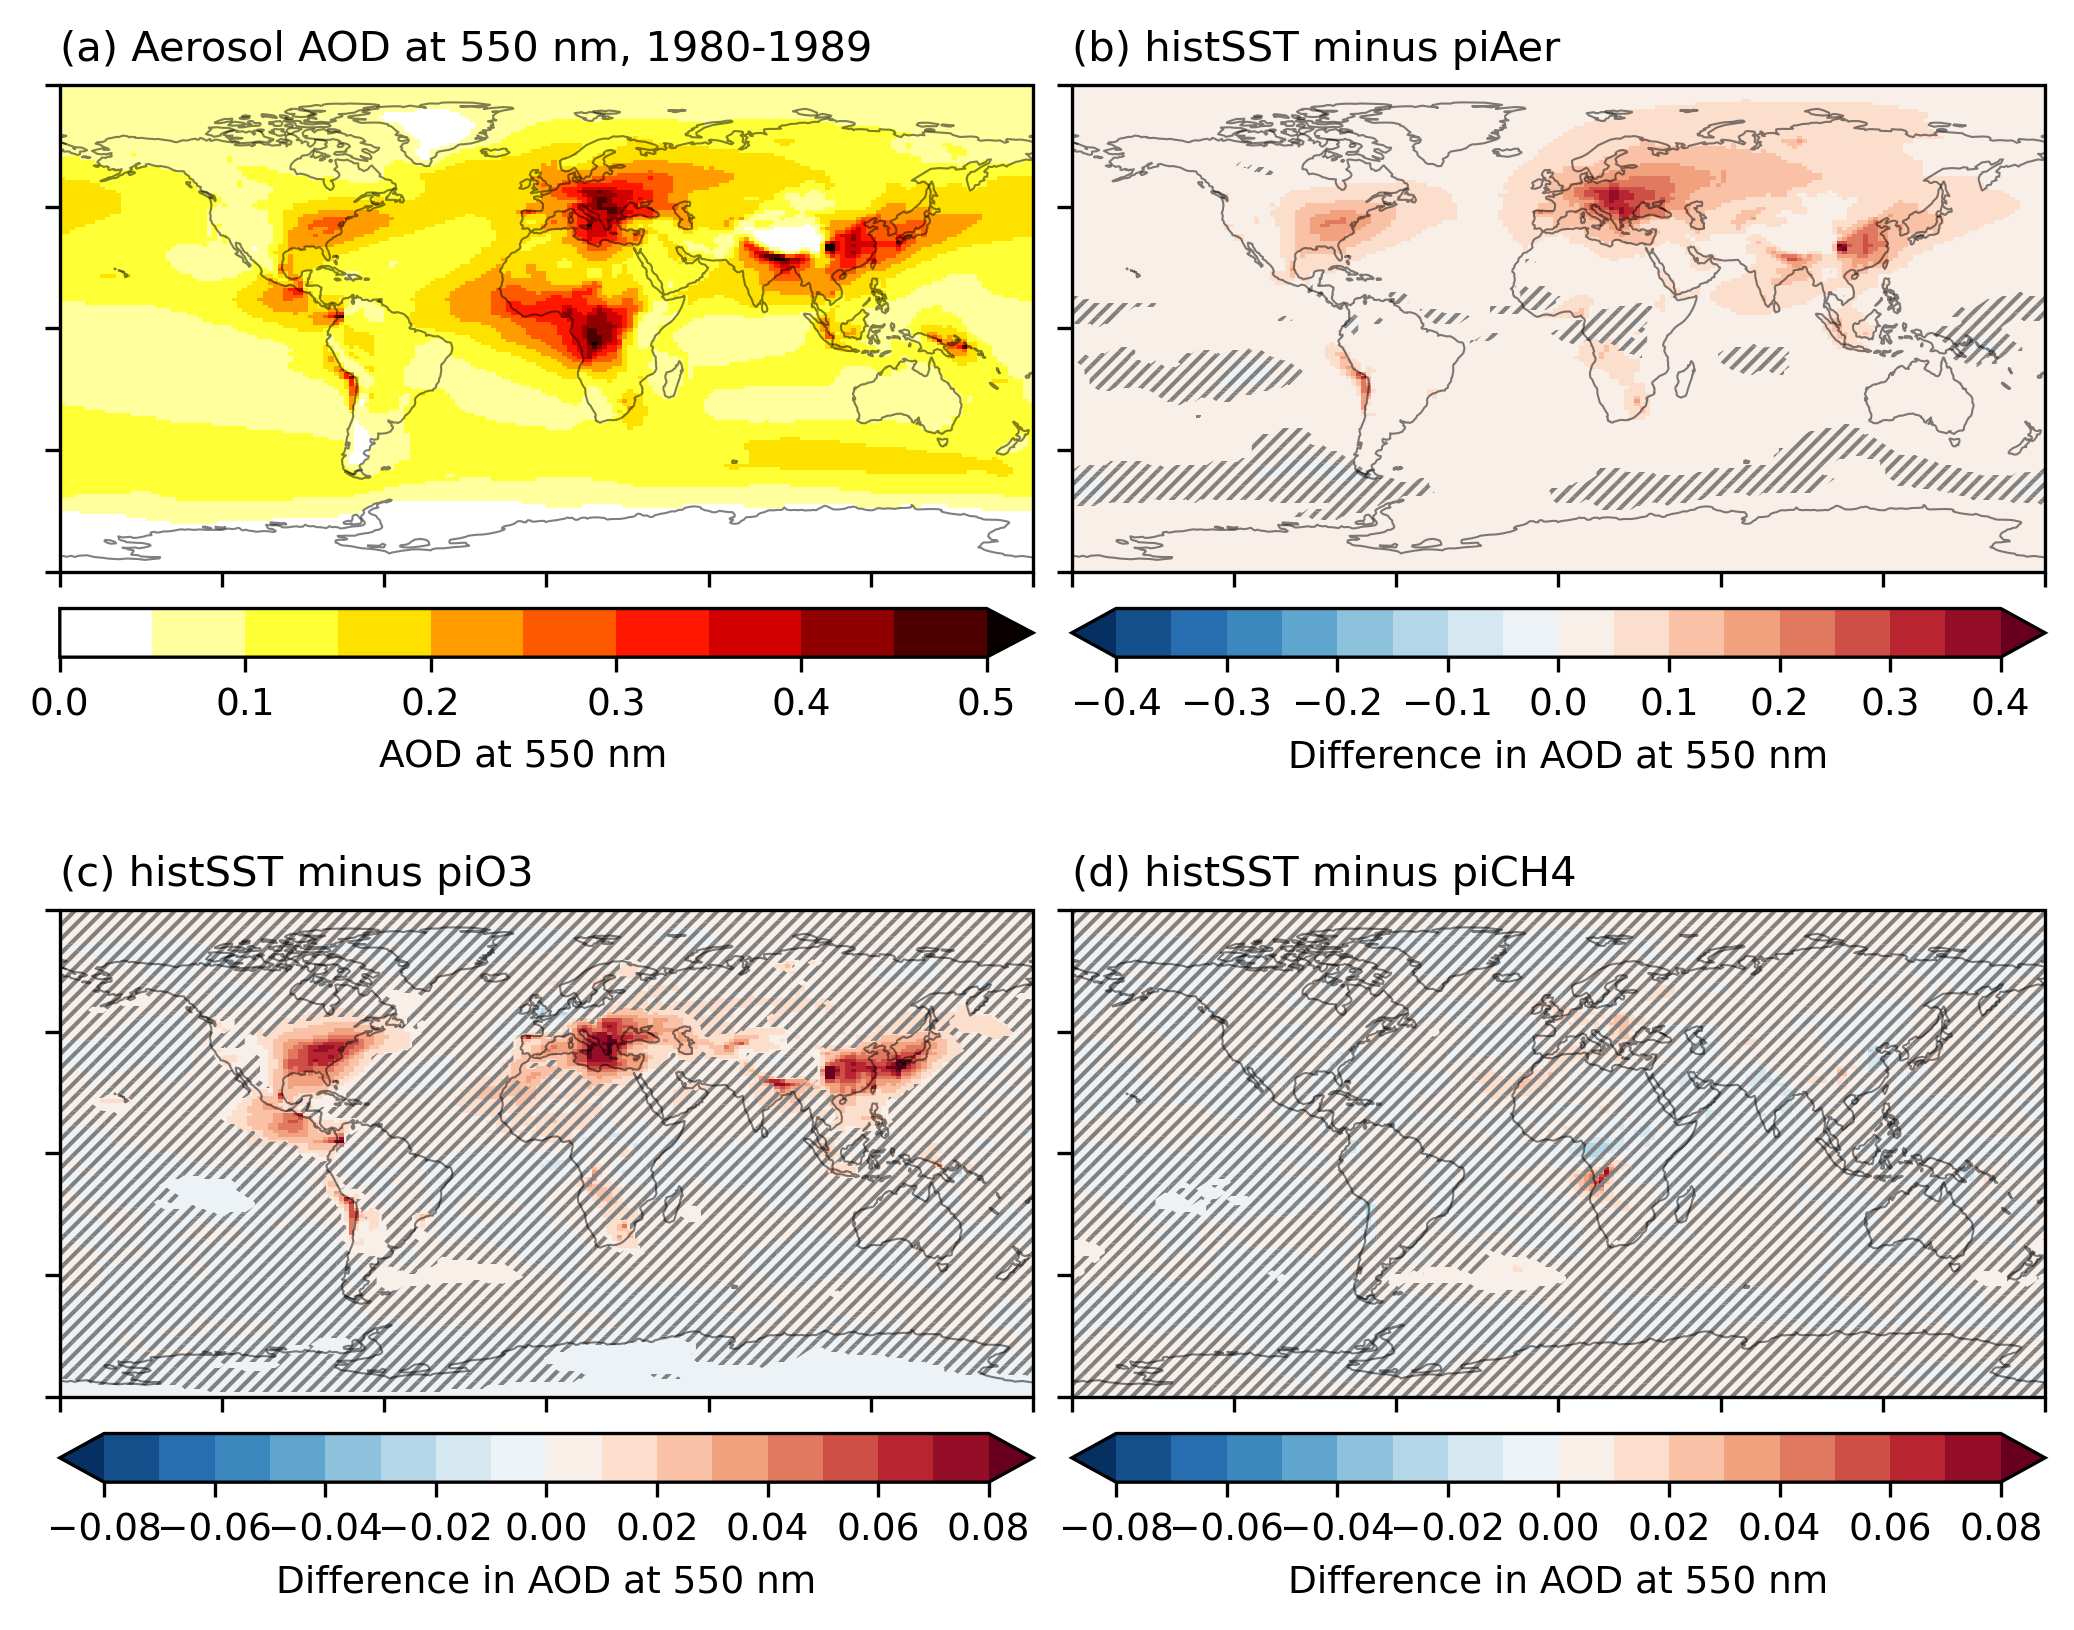
\includegraphics[width=\linewidth]{Chapter3/Figs/f06_aod-map.png}
    \caption{(a) Decadal mean aerosol AOD at 550 nm from 1980-1989. (b-d) Difference of aerosol AOD at 550 nm from 1980-1989 between histSST and histSST-piAer, histSST-piO3, and histSST-piCH4, respectively. Hatched areas denote areas in which the difference is not statically significant (p<0.05)}
    \label{fig:AOD-map}
\end{figure}


Figure \ref{fig:AOD-map} shows the location of AOD changes due to oxidants. There is a localised increase of AOD in the high emission areas such as Northern America, Central Europe, and Eastern Asia due to aerosol precursor emissions in the 1980s. \ce{O_3} precursors are responsible for 20\% of AOD in these areas (0.08 out of 0.4 over the European region, for example). \ce{CH_4} has an insignificant effect on AOD. This shows that although a global change of reaction tendency was observed, it may not be reflected in some aerosol diagnostics such as AOD. This is due to the nullifying nature of the change: increase of \ce{SO_2 - OH} oxidation and the decrease in \ce{SO_2 - H_2O_2} which results in net zero change in total oxidation tendency compared to histSST. We note here that anthropogenic \ce{CH4} is shown, in the next section, to affect cloud properties.

% Compare the AOD evaluation in Mulcahy and also discuss the updated AOD from Hardarcre and UKESM1.1
\citet{mulcahyDescriptionEvaluationAerosol2020} have evaluated AOD simulated by the UKESM1 against both ground-based measurements and satellite retrievals and found good agreement in trends but underestimated the absolute values. They found that the global annual mean AOD trends from AMIP simulation between 1980-2015 show an overall increase in AOD which is consistent with the Collection 6 MODIS merged dataset (MODIS C6) satellite retrieval. The absolute AOD is underestimated by 0.03 but is still within the lower end of the range of the satellite AOD. The spatial distribution shows that the UIKESM1 has higher AOD in the winter seasons of each hemisphere. This is due to the high sea-salt emission which peaks in the winter months. The high bias in sea-salt AOD does not affect our analysis which subtracts AOD from piAer, piO3 and piCH4 with histSST.

% discuss the updated effect of dry deposition from UKESM1 with UKESM1.1
The UKESM1 was updated with a new dry deposition scheme which affects the predicted aerosol AOD \citep{mulcahyUKESM1DevelopmentEvaluation2022}. The new version of UKESM1, the UKESM1.1, predicted a lower aerosol AOD, with a difference of at least 0.02 starting from 1980 due to a higher \ce{SO_2} dry deposition which removes \ce{SO_2} from the atmosphere, leaving less to oxidise to form \ce{SO_4}. This new dry deposition scheme further increases the low bias in \ce{SO_4} concentration compared to measurements. The annual mean OAD from UKESM1 and UKESM1.1 over 2003-2014 shows that the global mean AOD predicted by the models are 0.137 and 0.146, respectively, which are lower than most satellite measurements from MODIS (0.162), ORAC (0.170) and Swansea (0.135). These products, their uncertainties and details of the evaluation procedure are described in detail in \citet{mulcahyDescriptionEvaluationAerosol2020}. The spatial increase in the AOD in UKESM1.1 stems from the revised dust tuning which increases the dust AOD over and downwind of major dust source regions. This update is not relevant to \ce{SO_2} oxidation. However, there is a decrease in AOD in UKESM1.1 over China due to an increase in \ce{SO_2} dry deposition. Our work used output from the original UKESM1 thus the AOD will have a less low bias in absolute AOD and higher overall \ce{SO_4} loading.



\subsubsection{Aerosol size distribution}
\label{sec:result:aerosol-size-dist}

\begin{figure}
    \centering
    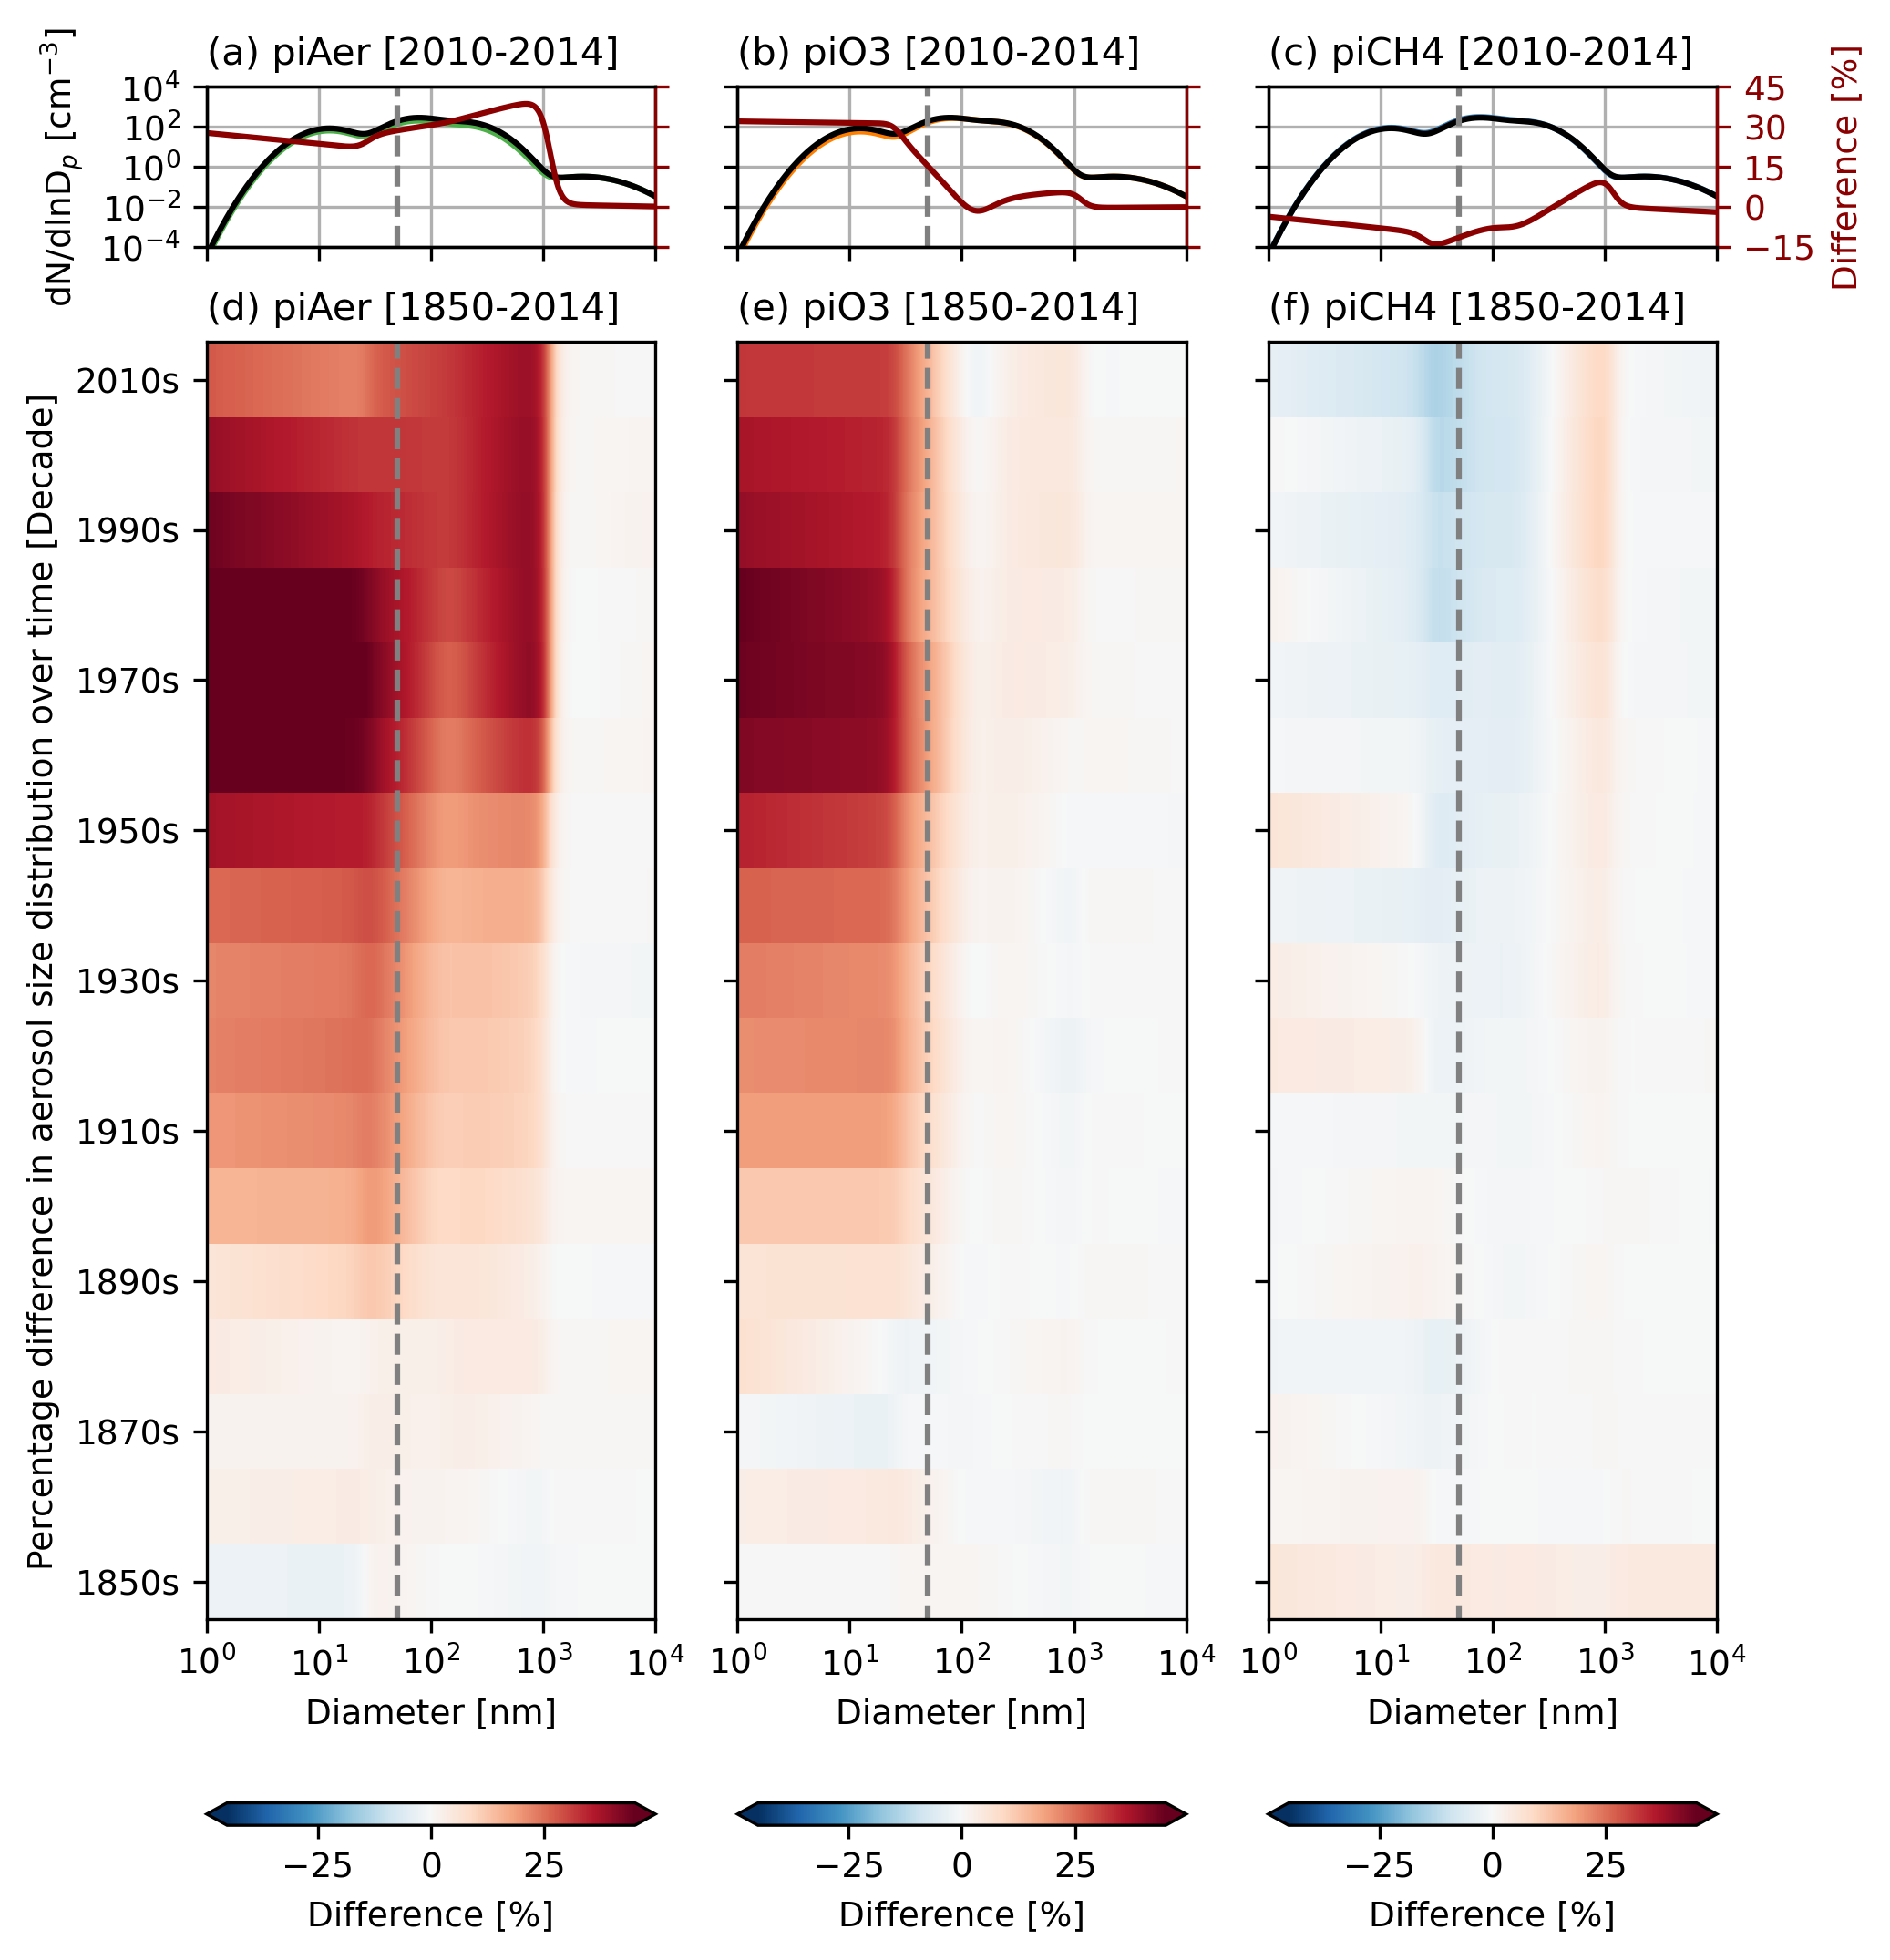
\includegraphics[width=\linewidth]{Chapter3/Figs/f08_aerosol-size-dist-over-time.png}
    \caption{(top) Historical total aerosol size distribution at 1 km for 2010-2014 with percentage difference on the secondary axis. (bottom) The progression of percentage change of aerosol size distribution due to (d) aerosol precursors (e) \ce{O_3} precursors and (f) \ce{CH4}. The vertical dashed line denotes the 50 nm diameter above which aerosol affects cloud nucleation.}
    \label{fig:aerosol-size-dist-time}
\end{figure}


Perturbation to oxidants modifies global aerosol size distribution over the historical period. The top panels of figure \ref{fig:aerosol-size-dist-time} show aerosol size distribution and percentage differences between histSST and the piAer, piO3 and piCH4 simulations for 2010-2014 at 1 km. The bottom panels show the progression of change in aerosol size over time. In panels (d - f), each horizontal bar denotes the percentage difference of global decadal mean aerosol size distribution at 1 km between histSST and the perturbed simulations. For example, the percentage differences for 2010-2014 in figures (a-c) are plotted as the topmost colour bar in figures (d-f). 

As shown by figure \ref{fig:aerosol-size-dist-time}d, historical aerosol precursor emissions increase aerosol concentrations with diameters smaller than 50 nm by more than 40\%  between the 1960s and 1980s. The number of particles greater than 50 nm in diameter (N50 -- dashed grey vertical line) has increased by 30-35\% and this is likely to affect the concentration of cloud condensation nuclei (CCN) (ref which talks about this. Seinfeld and Pandis?). In contrast, historical \ce{O_3} precursors increase the concentration of particles with a diameter of less than 50 nm by 30\% but only increase the concentration of particles with a diameter above 50 nm by 4\%. As shown in Section \ref{sec:oxidation}, the \ce{O_3} precursors affect only the \ce{SO_2 + OH} reaction tendency which forms new sulfate aerosol particles. The piCH4 shows that the historical increase in \ce{CH_4} leads to an increase in the aerosol concentration with a diameter above 1000 nm by 8\% after 1970s; however, the concentration of aerosol at this size is negligible, with only 1-2 particles per cm${^3}$. More importantly, \ce{CH_4} decreases the aerosol concentration up to 300 nm diameter as the increase in \ce{CH_4} decreases the \ce{SO_2 + OH} reaction tendency which contributes to new aerosol formation. 

% add discussions on the results by O'Connor
The change in aerosol size distribution due to \ce{CH_4} were mentioned in \citep{oconnorApportionmentPreIndustrial2022}. They found that an increase in \ce{CH_4} concentration in the present day leads to a significant reduction in aerosol number concentration in Aitken and accumulation mode. The reduction in N50 occurs across all latitudes and through the depths of the atmosphere. As \citet{oconnorApportionmentPreIndustrial2022} used timeslice simulations in their work, our work adds to their finding that the reduction in N50 occurs as early as the 1920s and increases in magnitude over time, to a maximum relative difference of 15\% in 2010. 

\subsection{Cloud properties}

\begin{figure}
    \centering
    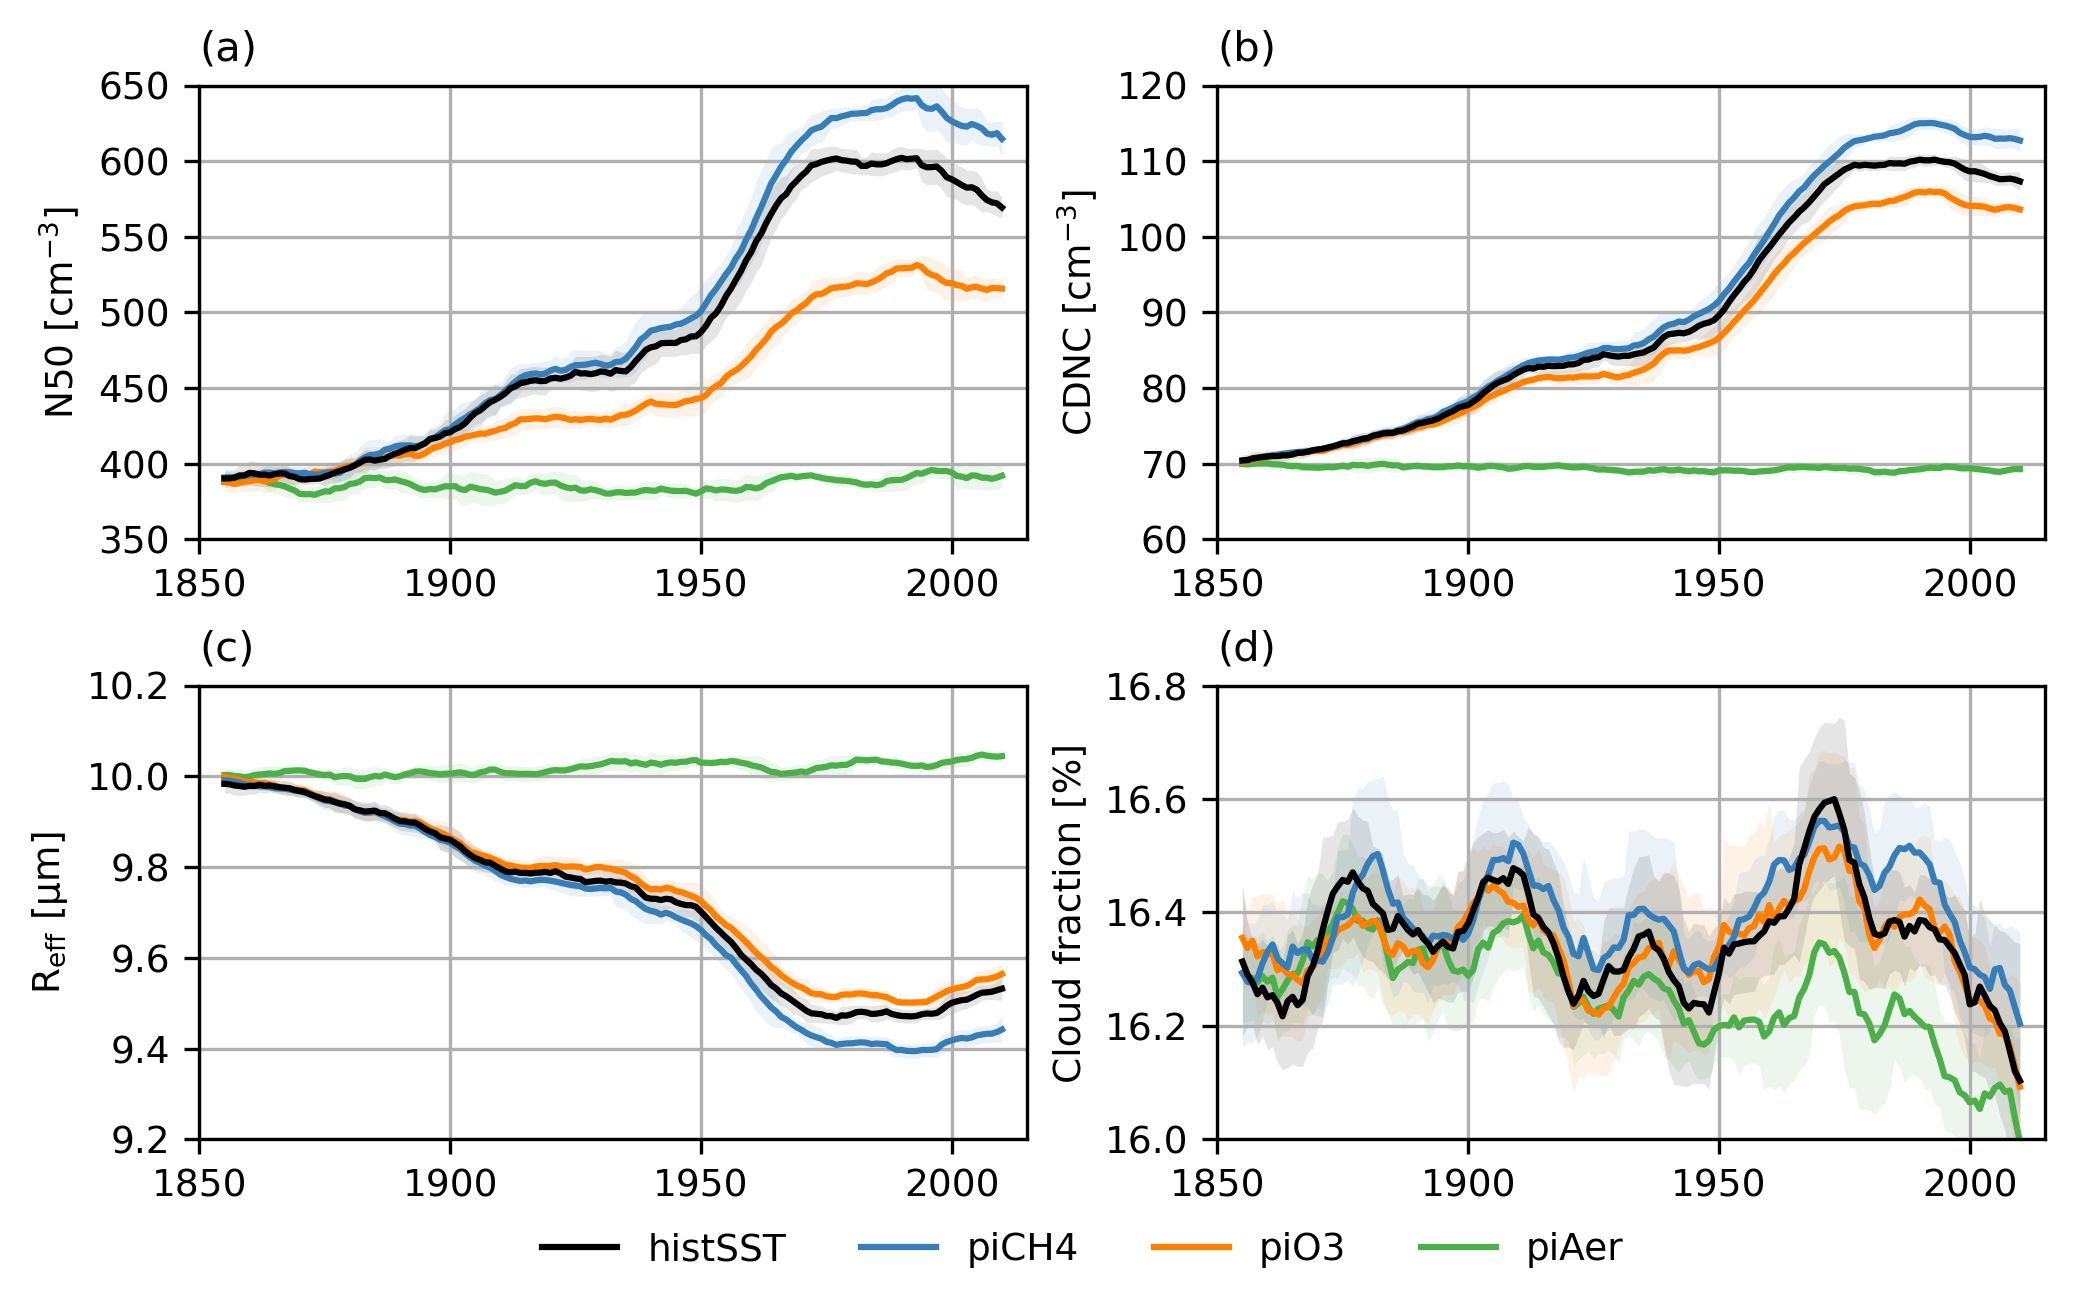
\includegraphics[width=\linewidth]{Chapter3/Figs/f09_cloud-props.png}
    \caption{Change in annual mean (a) concentration of particles greater than 50 nm diameter (N50), (b) cloud droplet number concentration (CDNC), (c) effective cloud droplet radius (R$_{\textrm{eff}}$) and (d) cloud fraction at 1 km. A 10-year rolling mean was applied to the data. Shaded areas denote the standard deviation from the 10-year mean.}
    \label{fig:cloud}
\end{figure}

Aerosols with a diameter above 50 nm (N50) act as cloud condensation nuclei in which their concentration modifies cloud properties. Figure \ref{fig:cloud} shows the global decadal mean N50 concentration as well as cloud properties including cloud droplet number concentration (CDNC), cloud droplet effective radius (R$_{eff}$) and cloud fraction at 1 km. It shows that N50 rises from 400 cm$^{-3}$ in 1850 to 600 cm$^{-3}$ in the 1980s then decreases slightly in the historical period. This trend is in line with cloud properties change. \ce{O_3} precursors are responsible for 12.5\% (75 cm$^{-3}$  of 600 cm$^{-3}$) of total N50 in 1980s. Meanwhile, an increase in N50 in piCH4 implies that historical anthropogenic methane emissions lower N50 concentration.

Cloud properties show signs of changes due to aerosol precursors and oxidant changes. Figure \ref{fig:cloud}b shows global mean cloud properties at 1 km above ground. CDNC increases by 40 cm$^{-3}$ due to aerosol precursors. \ce{O_3} precursors increase CDNC while \ce{CH_4} decreases CDNC. This is linked to the change in \ce{SO_2 + OH} reaction tendency as this reaction increases aerosol number in the atmosphere, which will affect CDNC \citep{twomeyInfluencePollutionShortwave1977}. While AOD, seen in figure \ref{fig:AOD-map}, does not indicate a significant change due to \ce{CH_4}, cloud properties show a clear increase to CDNC and a decrease to R$_{eff}$. This is in line with work done by \citet{karsetStrongImpactsAerosol2018}, which found that the distribution of the changes in aerosol number concentration does not always correspond directly to the distribution of the changes in cloud and radiative properties. In essence, historical \ce{CH_4} increases the cloud effective radius and decreases CDNC.

Cloud fraction increases by 0.2\% due to aerosol precursors. However, \ce{O_3} and \ce{CH_4} do not significantly alter cloud fractions as shown in \ref{fig:cloud}c. 




\subsection{Radiative effects}

Greenhouse gases, aerosols and clouds could perturb the Earth's radiative balance. One way to quantify the effect of each of the forcings is via the decomposition of effective radiative forcing (ERF) as described in section \ref{sec:erf}. The ERF is decomposed into the clear and clean sky part or $ERF_{cs,clean}$, the aerosol instantaneous radiative forcing (i.e., scattering and absorption) or aerosol IRF, and the cloud radiative effect or the $\Delta CRE'$. Here we show that \ce{O_3} precursors affect aerosol IRF and that \ce{CH_4} affects cloud radiative effect.

\begin{figure}
    \centering
    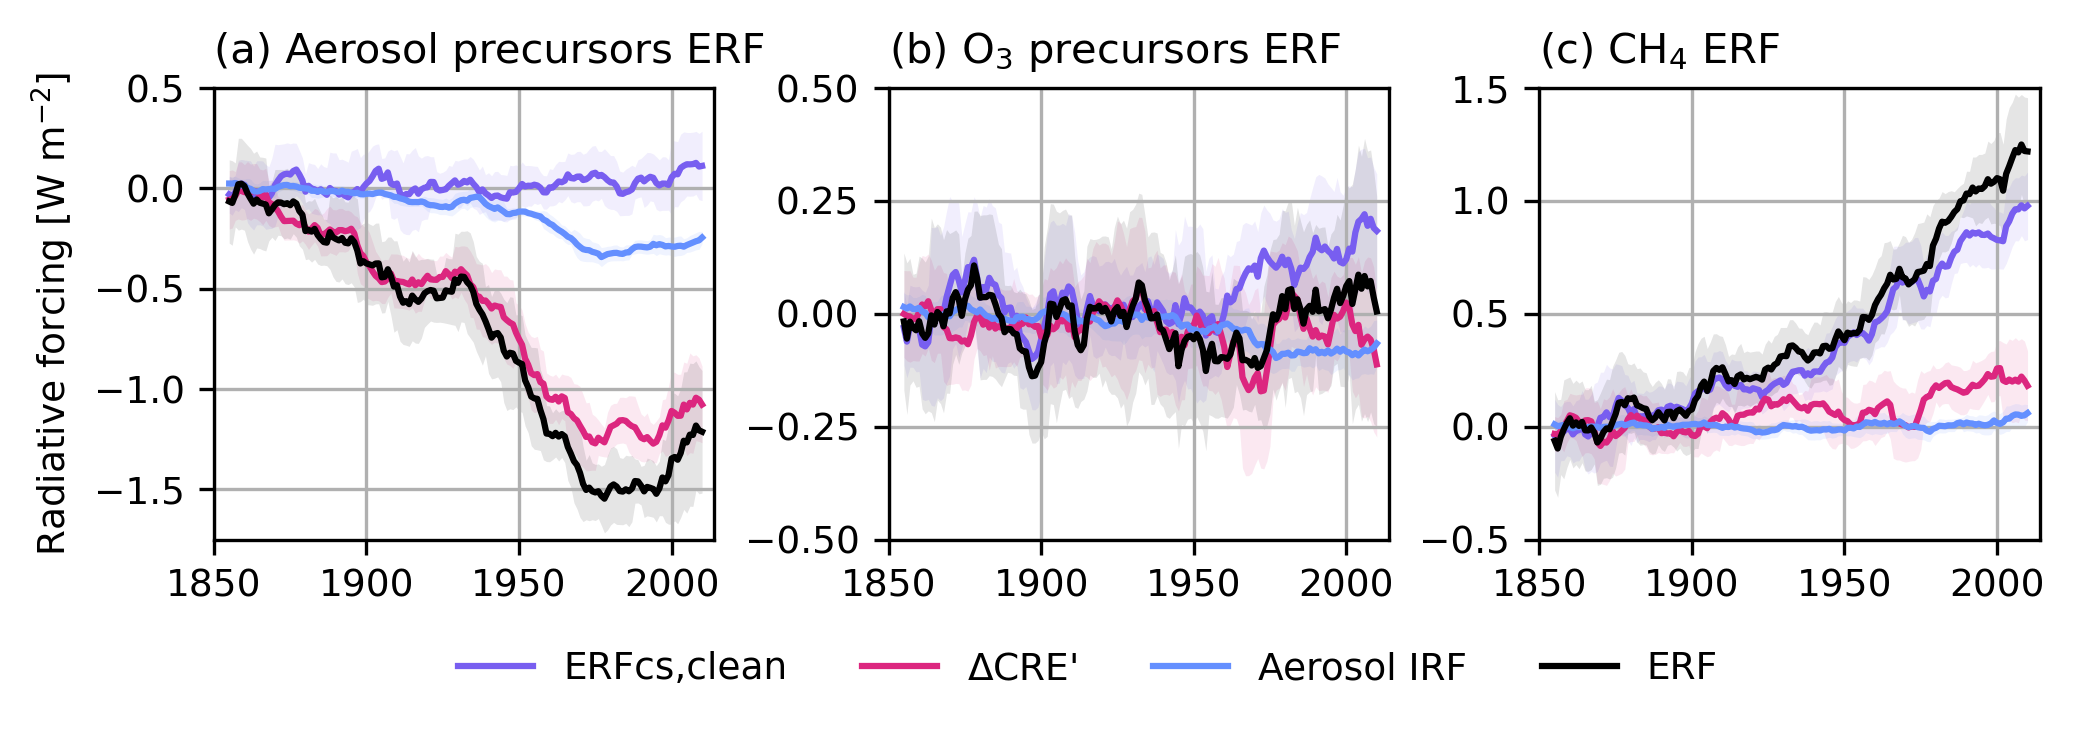
\includegraphics[width=\linewidth]{Chapter3/Figs/f10_erf.png}
    \caption{Global mean aerosol radiative forcing due to (a) aerosol precursors, (b) \ce{O_3} precursors and (c) \ce{CH_4}. A 10-year rolling mean was applied to the data. Shaded areas denote the standard deviation from the 10-year mean.}
    \label{fig:erf}
\end{figure}
% sstpiaer
% irf -0.2772347016768022
% irf_std 0.031058704
% cre -1.0905492262406782
% cre_std 0.19105731
% sstpio3
% irf -0.08279982263391668
% irf_std 0.05211312
% cre -0.04306954470547763
% cre_std 0.16057429
% sstpich4
% irf 0.039096790010278874
% irf_std 0.037890494
% cre 0.21275067762895067
% cre_std 0.15470749

Figure \ref{fig:erf} shows the global annual mean aerosol ERF from aerosol precursors, \ce{O_3} precursors and \ce{CH_4}. Figure \ref{fig:erf}a shows that aerosol precursors contribute mostly to the cloud radiative effects (-1.01$\pm$0.19 W m$^{-2}$), followed by aerosol IRF (-0.18$\pm$0.04 W m$^{-2}$). Aerosol precursor ERF is highest between 1970-1990 due to an increase in both cloud radiative effect and instantaneous radiative forcing. Aerosol precursors include absorbing aerosols such as black carbons which contribute to net positive IRF in some regions such as eastern central China \citep{seoImpactsAerosolEmissions2020, oconnorAssessmentPreindustrialPresentday2021}. 


\ce{O_3} is an important greenhouse gas \citep{forsterEarthEnergyBudget2021}. By itself, the present-day change in \ce{O_3} has a positive (warming) clear-sky radiative forcing of 0.25 W m$^{-2}$ compared to 1850. There is a slight decrease in aerosol IRF due to \ce{O_3} precursors starting in the 1960s and up to 0.08$\pm$0.05 W m$^{-2}$ between 2000-2014. This is due to the increase in new aerosol formation from the \ce{SO_2 + OH} reaction tendency since the amount of scattered solar radiation is proportional to the total column mass burden of particles \citep{nemesureDirectShortwaveForcing1995}. We see that from Figure \ref{fig:AOD-map}, there is a statistically significant change to AOD due to \ce{O_3} precursors. There is no clear change to cloud radiative effects due to \ce{O_3}, consistent with \citet{skeieHistoricalTotalOzone2020}, who reported that cloud adjustments due to \ce{O_3} are in the order of 0.02 W m$^{-2}$. However, we note that the UKESM1 is the only model with troposphere and stratosphere chemistry the gives negative ERF in the present-day \citet{skeieHistoricalTotalOzone2020}. 

\ce{CH_4} is a greenhouse gas that also affects the cloud adjustment \citep{oconnorApportionmentPreIndustrial2022}. The increase in \ce{CH_4} in the present-day has resulted in an increase in the clear-sky radiative forcing of 1.0 W m$^{-2}$ since 1850. Changes in \ce{CH_4} since 1850 have resulted in negligible changes in the aerosol direct effect. This is due to the reaction tendency of \ce{SO_2 + OH} and \ce{SO_2 + H_2O_2} roughly cancelling out, resulting in an unchanged aerosol loading as shown in the aerosol AOD, figure \ref{fig:AOD-map}. On the other hand, the decrease to CDNC and increase in cloud droplet effective radius from 1850s to historical \ce{CH_4} results in a positive cloud radiative effect of 0.21$\pm$0.15 W m$^{-2}$. These results agree with the time slice study reported in \citep{oconnorApportionmentPreIndustrial2022}.

% discuss oconnor in details
\citet{oconnorApportionmentPreIndustrial2022} showed that the increase in \ce{CH_4} concentration leads to changes to aerosol properties, which leads to a positive total \ce{CH_4} ERF. Their study used two timeslice experiments: pre-industrial and pre-industrial with present-day \ce{CH_4} to calculate the aerosol ERF. The ERF estimates suggest that the total \ce{CH_4} ERF from UKESM1 includes a significant indirect contribution from aerosols. The direct CH4 ERF at the present-day relative to the preindustrial period is 0.85$\pm$0.03 W m$^{-2}$ \citep{oconnorAssessmentPreindustrialPresentday2021}.

% Discuss Thornhill 2021 (Multi model Aerosol ERF calculation from different NTCF including CH4 and O3 - See Table 5)



\section{Conclusions}

Changes in oxidants due to \ce{O_3} precursors and \ce{CH_4} affect sulfate aerosol formation, cloud formation and ultimately aerosol ERF, but the impacts of oxidants on ERF are not well understood. In this work, we used results from AerChemMIP experiments to investigate the effects of oxidant changes on sulfate aerosol formation, aerosol and cloud properties and aerosol effective radiative forcing. By looking at the change in gas phase oxidation, we can identify a net negative change to IRF by \ce{O_3} and a net positive change by \ce{CH_4} to CRE. These changes ... 

% Effects due to O3
Historical \ce{O_3} precursor emissions increase \ce{O_3} mixing ratio as well as \ce{OH} and \ce{H_2O_2}. These oxidant increases enhance the \ce{SO2 + OH} reaction tendency and significantly increase the aerosol AOD near high \ce{SO_2} emission regions.  Due to \ce{O_3} precursors, the concentration of aerosols with size below 50 nm increases, which increases the cloud droplet number concentration. Ultimately, ozone precursors increase the aerosol instantaneous radiative forcing by up to 0.08$\pm$0.05 W m$^{-2}$ between 2000-2014, which is 44\% of aerosol IRF due to aerosol precursors, further cooling the climate.

% Effects due to CH4
On the other hand, \ce{CH_4} decreases the OH concentration as \ce{CH_4} acts as an OH sink. Increases in \ce{CH_4} also increases \ce{H_2O_2} and \ce{O_3} mixing ratios. These changes in oxidants decrease the OH reaction tendency (\ce{SO_2 + OH}) but increase the \ce{SO_2 + H_2O_2} reaction tendency, resulting in an unchanged sulfate budget but a larger mean aerosol diameter as the \ce{H_2O_2} oxidation occurs in the liquid phase where aerosol growth occurs more easily. This change in aerosol size distribution minimises CDNC and enhances the effective cloud droplet radius. As a result,\ce{CH_4} contributes to a positive cloud radiative effect of 0.21$\pm$0.15 W m$^{-2}$ between 2000-2014, further adding to the warming impact of methane on the climate.

Changes in aerosol precursor emissions have had an important impact on the climate offsetting a significant fraction of the warming from long-lived greenhouse gases. However, we've shown here that accounting for oxidants over the historical period is important to accurately simulate sulfate aerosol formation and the resulting aerosol radiative effects. Up to 40\% of the change in ....  
